% Algemene settings
\documentclass{beamer}
\usepackage[dutch]{babel}
\usepackage{graphicx}
\graphicspath{{img/}}


% Thema en stijl
\usetheme{Madrid}
\usecolortheme{whale}
\beamertemplatenavigationsymbolsempty
\setbeamertemplate{itemize items}[circle] 


% ToC aan begin elke subsectie (indien te vaak verander
% naar section)
\AtBeginSection[]
{
  \begin{frame}<beamer>{Inhoud}
  \small
    \tableofcontents[currentsection]
  \end{frame}
}


% Title page
\title[Capaciteitsproblemen ticketsector]{\Huge{Capaciteitsproblemen bij online ticketverkoop}}
\author[Groep 2]{Sonia Amiri \and Rami Berro \and Florian Braùn \and Tom Cottem \and Thijs Creemers \and John Cai \and Lode Dockx}
\date[Informaticawerktuigen]{\small{Informaticawerktuigen - 29 november 2023}}
\logo{
\includegraphics[height = 1cm]{kul-logo.png}}


% Start slides
% TEKST VAN ELK DEEL MAG 1m20 DUREN
\begin{document}


% TEKST INTRODUCTIE
% =================
% Goedemiddag.
% Onze presentatie zal gaan over capaciteitsproblemen bij online diensten.
% Het gaat daarbij over de overbelasting van servers, waardoor allerhande problemen kunnen
% optreden zoals onbereikbaarheid van websites.
% We gaan daarbij een focus leggen op de verkoop van online concerttickets.
\begin{frame}
  \titlepage
\end{frame}


\section[Intro]{Introductie}
% TEKST INTRODUCTIE
% =================
% De concrete aanleiding voor deze bespreking is de verkoop van tickets voor Taylor
% Swift-concerten in 2022.
% Die verkoop verliep chaotisch doordat veel fans tegelijkertijd de website van het bedrijf
% Ticketmaster wilden raadplegen, wat storingen veroorzaaktte en leidde tot ophef
% die zodirect dieper zal worden besproken.
% Het is vooral belangrijk dat dit helemaal geen alleenstaand geval is. Capaciteits-
% problemen duiken vaker op, ook in andere sectoren.
% De gevolgen kunnen bovendien groot zijn: zoals inkomstenverlies indien klanten niets
% kunnen kopen, schade aan imago, ontrevredenheid, en zelf veiligheidsrisico's indien
% burgers bij bv. een ramp een overheidswebsite niet kunnen raadplegen
% Het is daarom ook belangrijk om na te gaan hoe dit kan worden vermeden, zowel
% voor de verkoop van tickets, als in andere domeinen.
\begin{frame}{Introductie}
    \begin{itemize}
        \item Chaos bij ticketverkoop Swift: capaciteitsproblemen bij Ticketmaster
        \item Geen alleenstaand geval: oook bij andere online diensten
        \item Mogelijke gevolgen: inkomstenverlies, imagoschado, ontevredenheid,
        veiligheidsrisico's ...
        \item Dus: nagaan hoe dit kan worden vermeden, zowel in
        ticketverkoop, als daarbuiten
    \end{itemize}
    \begin{center}
        
\includegraphics[height = 2.5cm]{ticketmaster-logo.png}
        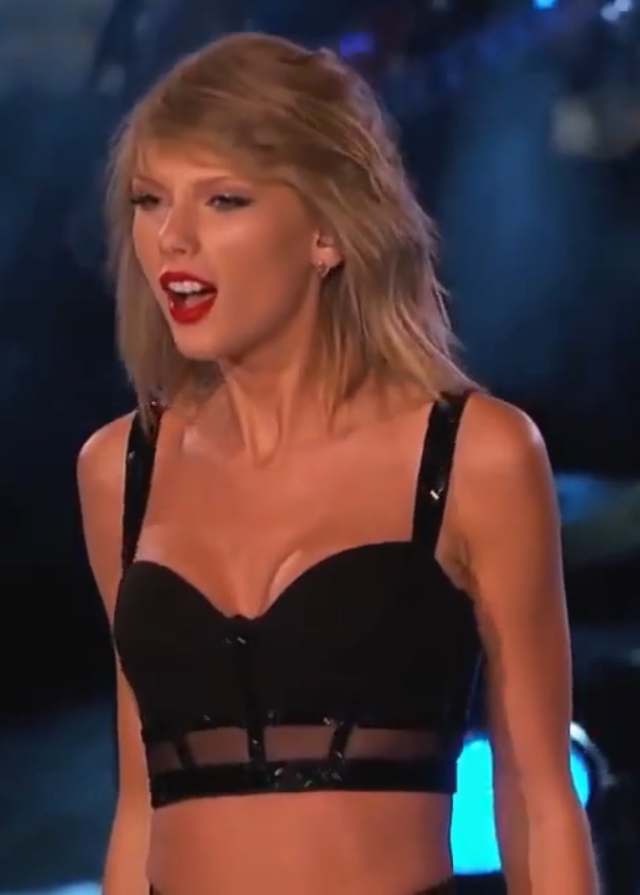
\includegraphics[height = 2.5cm]{taylor-swift.png}
        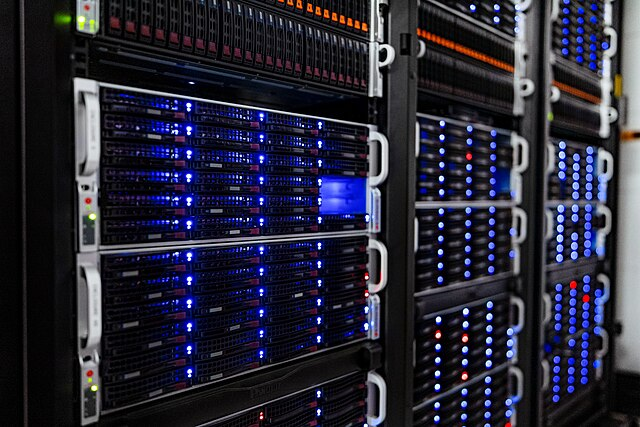
\includegraphics[height = 2.5cm]{server-rack.jpg}
    \end{center}
\end{frame}


% TEKST INTRODUCTIE
% =================
% Hier kunnen jullie het overzicht zien van wat we zullen bespreken in deze presentatie
% We gaan eerst wat dieper in op de actualteitsproblemen in de ticketverkoop
% Daarna geven we een technische bespreking van capaciteitsproblemen en mogleijke oplossingen
% En daarna gaan we, voor de ticketsector, de belangen van bedrijven en
% klanten bespreken
% En gaan we ook in op het eventuele machtsmisbruik van de ticketverkoopbedrijvne
%  en wat daartegen kan worden ondernomen.
\begin{frame}{Inhoud}
  \tableofcontents
\end{frame}


\section[Actualiteitsproblemen]{Actualiteitsproblemen ticketsector}
% TEKST ACTUALITEITSPROBLEMEN
% ============================
% Ticketmaster werd recentelijk bekritiseerd door de uitverkoop van Taylor Swift's Eras Tour in november 2022. 
% Deze tour werd voorspeld als een van de best verkochte in de geschiedenis, als de comeback na Swift's eerdere succesvolle
% Reputation-wereldtournee. Ticketmaster meldde meer dan 14 miljoen bezoekers op hun site tijdens de voorverkoop, maar beweerde slechts
% 1,5 miljoen toegangscodes te hebben uitgegeven. Fans waren verontwaardigd over lange wachttijden, een haperend systeem, tekort aan
% tickets en abrupte prijsstijgingen. Politiek gezien riep vertegenwoordiger Alexandria Ocasio-Cortez op tot verzet tegen Ticketmaster
% en benoemde het een monopolie door de fusie met LiveNation, waarbij de enorme prijsstijgingen en wachtrijen als voornaamste redenen
% werden aangehaald. Met meer dan 70% controle op de markt, kan Ticketmaster zijn macht misbruiken zonder concurrentie, zoals duidelijk
% werd tijdens de uitverkoop van de Eras Tour.
% Later volgde er ook in hoorzitting in de Amerikaanse senaat over de situatie in de sector en 
% de positie van LiveNation/Ticketmaster.
\begin{frame}{Actualiteitsproblemen ticketsector}
    \begin{itemize}
        \item Taylor Swift - Eras Tour
        \item Verwachtte best verkochte tour
        \item Fans woedend door lange wachttijden, hoge prijzen ...
        \item Politieke backlash
        \item Kritiek op marktpositie Ticketmaster
    \end{itemize}
    \begin{center}
        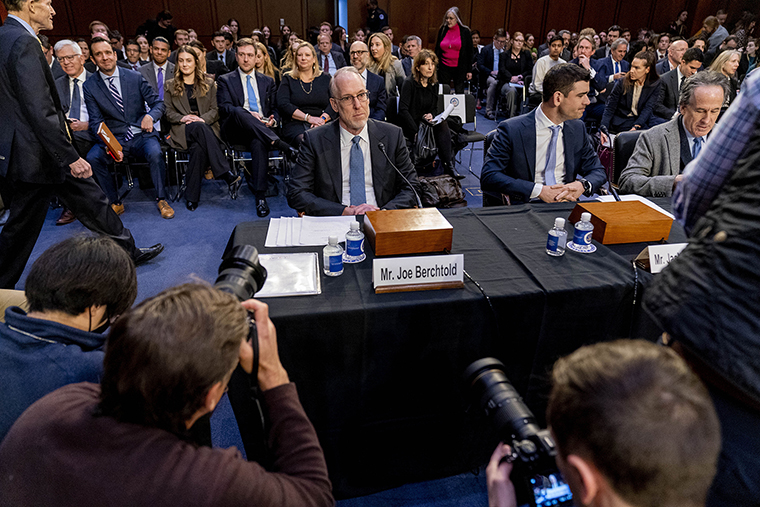
\includegraphics[height = 2.5cm]{senate-hearing.jpg}
        
\includegraphics[height = 2.5cm]{frustratie.png}     
    \end{center}
\end{frame}


\section[Capaciteitsproblemen]{Capaciteitsproblemen bij overbelasting online diensten}
% TEKST CAPACITEITSPROBLEMEN
% ==========================
% Deze sectie zal technischer zijn. We gaan ingaan op wat capaciteitsproblemen precies zijn
% en wat mogelijke oplossingen zijn. Dit is iets dat van toepassing is op alle mogelijke online diensten.
% Dus dit staat meer los van ticketverkoop.
% 
% Er is sprake van een capaciteitstekort wanneer de server of servers onvoldoende resources
% hebben om de inkomende verzoeken af te handelen. Deze inkomende verzoeken ontstaan doordat
% gebruikers de server(s) van een website of dienst proberen te bereiken.
% 
% Indien er te veel verzoeken zijn voor de resources die op een bepaald moment beschikbaar
% zijn kunnen er verschillende gevolgen optreden. Het gaat dan bv om langere laattijden,
% applicaties die vreemde beginnen te functioneren, of errorcodes in de browser.
% 
% Oorzaken van een te grote hoeveelheid aan verzoeken kunnen verschillend zijn:
% het kan zijn dat de standaardcapaciteit ontoereikend is, dat er pieken zijn in gebruik
% bv. door een online actie op een bepaalde site, of dat servers overbelast worden door
% cyberaanvallen of web scraping.
% 
% Er bestaan verschillende manieren om deze problemen aan te pakken. We lichten er aantal
% toe:
% - Eerst en vooral kan men opschalen door krachtigere servers te voorzien of een groter
% aantal servers, waarover de werklast wordt verdeeld
% - Verder kan men proberen om het gebruik van zogenaamde cache te verbeteren, waarbij
% veel data die vaak wordt opgevraagd op snellere opslag bewaard wordt
% - Verder kan men de software code proberen optimaliseren waardoor een app of site
% minder systeemresources gebruikt voor een bepaald verzoek af te handelen
% - Ook kan men beslissen om de inhoud van een site of app aan te passen tijdens
% piekbelasting door bv. minder informatie te tonen of de resolutie van afbeeldingen
% te verminderen
% - Men kan ook een stap verder gaan en beslissen om bepaalde componenten van de dienst-
% verlening volledig uit te schakelen om zo de essentiele dienstverlening te behouden
% (bv. resource-intesnieve recommendatiealgoritmes)
% 
% Daarnaast zijn er nog heel veel andere oplossingen, maar die kunnen we niet allemaal
% belichten tijdens de presentatie. Het gaat dan bv. over geografisch spreiden van
% servers of cache om connecties sneller te maken, automatisch opschalen van
% infrastructuur door gebruik van cloud-providers zoals amazon web services
% en automatische systeemconfiguraties waardoor extra servers snel kunnen worden
% ingeschakeld bij problemen
\begin{frame}{Capaciteitsproblemen bij overbelasting online diensten}
    
    Wat zijn capaciteitsproblemen?
    
    \begin{alertblock}{Capaciteitsproblemen}
        De serverinfrastructuur heeft onvoldoende systeemresources
        om alle inkomende verzoeken af te handelen
    \end{alertblock}

    \begin{columns}
        \column{0.60\textwidth}
            waarbij een verzoek onstaat doordat gebruikers server(s) proberen te bereiken
        \column{0.40\textwidth}
            \centering
            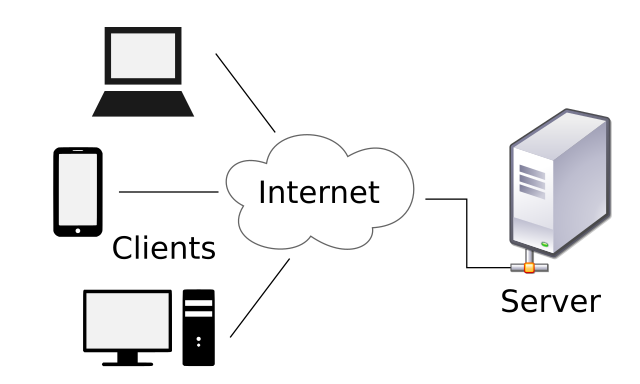
\includegraphics[width = \textwidth]{server-verzoeken.png}
    \end{columns} 

\end{frame}


\begin{frame}{Capaciteitsproblemen bij overbelasting online diensten}
    Mogelijke gevolgen:
    \begin{itemize}
        \item Tragere systemen
        \item Slecht functionerende systemen
        \item Niet meer functionerende systemen
    \end{itemize}
    \begin{center}
        
\includegraphics[height = 3cm]{destroy-computer.jpg}        
    \end{center}
\end{frame}


\begin{frame}{Capaciteitsproblemen bij overbelasting online diensten}
    Mogelijke oorzaken:
    \begin{itemize}
        \item Normaal gebruik
        \item Piekbelasting
        \item Onwenselijke verzoeken (bv. massale scraping)
        \item Cyberaanvallen (Denial of Service-aanvallen)
    \end{itemize}
    \begin{center}
        
\includegraphics[height = 3cm]{fluctuaties.png}
        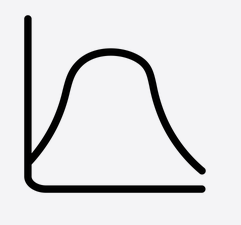
\includegraphics[height = 3cm]{piek.png}
        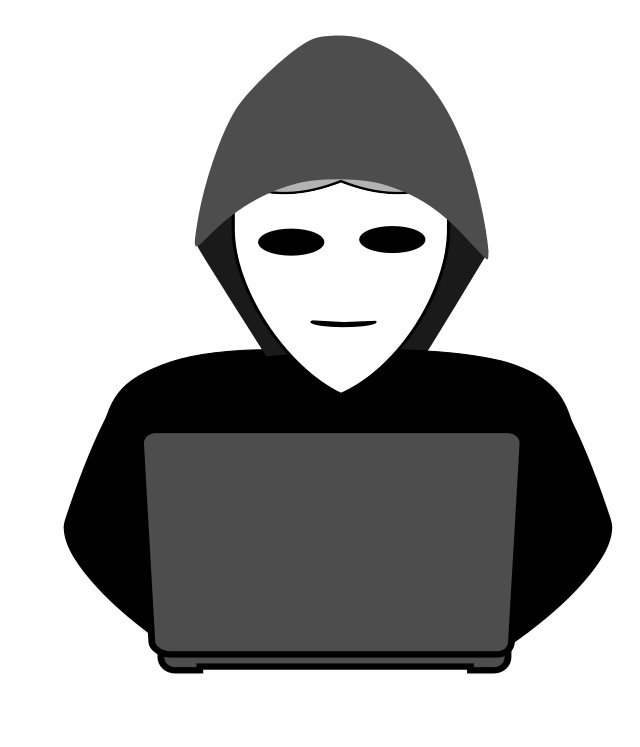
\includegraphics[height = 3cm]{hacker.png}        
    \end{center}
\end{frame}


\begin{frame}{Capaciteitsproblemen bij overbelasting online diensten}
    \Large{
        Mogelijke oplossingen
        \begin{itemize}
            \item Opschalen infrastructuur
            \item Cachen
            \item Optimaliseren algoritmen en datastructuren
            \item Adapteren site- of applicatieinhoud
            \item Selectief degraderen dienstverlening
            \item ...
        \end{itemize}
    }
\end{frame}


\begin{frame}{Capaciteitsproblemen bij overbelasting online diensten}
    \begin{center}
        \alert{\Huge{VEEL andere oplossingen!}}
    \end{center}
\end{frame}


\section[Bedrijfsbelangen]{Belangen van ticketsysteembedrijven}
% TEKST BEDRIJFSBELANGEN
% =======================
% Als we het hebben over de belangen van ticketsysteembedrijven, draait het voornamelijk om de marktsituatie, concurrentie, 
% winstmaximalisatie en het behoud van imago en merkreputatie.
% 
% Een dominante speler in de primaire ticketverkoop is Ticketmaster. Als primaire marktverkoper betekent dit dat 
% zij tickets rechtstreeks verkopen die aan hun zijn toegewezen door evenementpartners. Aan de andere kant, in de 
% secundaire markt, verkopen concurrenten zoals Eventbrite en StubHub reeds verkochte primaire tickets, meestal aan een hogere prijs.
% 
% Maar hoe streven deze bedrijven dan naar winstmaximalisatie? Hoewel concurrerende sites op het eerste gezicht mogelijk als 
% negatief worden beschouwd, is het tegendeel waar. Bijvoorbeeld, Live Nation, het moederbedrijf van Ticketmaster, heeft 
% juist de secundaire markt niet tegengewerkt, maar eerder een bedrijf op die markt, zoals TicketsNow, overgenomen.
%   
% Wanneer we spreken over imago en merkreputatie, kan een dergelijke actie leiden tot controverse, vooral omdat Ticketmaster 
% zelf beweerde maatregelen te nemen tegen de doorverkoop van tickets door de secundaire markt. Het behoud van hun imago is
% natuurlijk essentieel, en dit wordt bereikt door bijvoorbeeld afspraken na te komen met externe partijen zoals artiesten.
\begin{frame}{Belangen van ticketsysteembedrijven}
    \begin{itemize}
        \LARGE{
            \item Marktsituatie en concurrentie
            \item Winstmaximalisatie
            \item Imago en merkreputatie
        }
    \end{itemize}
\end{frame}


\begin{frame}{Marktsituatie en concurrentie}
    \begin{columns}
        \begin{column}{.6\textwidth}
            \begin{itemize}
                \LARGE{
                    \item Primaire ticketverkoper
                    \item Secundaire markt
                }
            \end{itemize}
        \end{column}
        \begin{column}{.4\textwidth}
            \begin{figure}
                
\includegraphics[width=50px,height=50px,keepaspectratio]{ticketmaster-logo.png}
            \end{figure}
            \centering
            
\includegraphics[width=45px,height=45px,keepaspectratio]{stubhub-logo.png}
            
\includegraphics[width=45px,height=45px,keepaspectratio]{eventbrite-logo.png}
        \end{column}
    \end{columns}
\end{frame}


\begin{frame}{Winstmaximalisatie}
    \begin{itemize}
        \LARGE{
            \item Andere sites = negatief?
            \item Live Nation
        }
    \end{itemize}
    \begin{center}
        
\includegraphics[height=50px, keepaspectratio]{livenation_logo.png}
    \end{center}
\end{frame}


\begin{frame}{Imago en merkreputatie}
    \begin{itemize}
        \LARGE{
            \item Maatregelen tegen misbruik secundaire markt?
            \item Hoe het imago behouden?
        }
    \end{itemize}
\end{frame}


\section[Gebruikersbelangen]{Belangen van klanten/gebruikers}
% TEKST GEBRUIKERSBELANGEN
% =========================
% Ticketsystemen hebben ten opzichte van de gebruiker voordelen en nadelen. Dit komt doordat er veel factoren komen kijken bij het maken van ticketsystemen. 
% deze voor- en nadelen kunnen de belangen van een klant toe- en tegenwerken.
% 
% De voordelen van een ticketsysteem zijn redelijk evident, maar zeker niet altijd heel merkbaar. Zo zijn ticketsystemen zeer gebruiksvriendelijk,
% ze worden ontworpen zodaning dat gebruikers zo gemakkelijk en efficiënt mogelijk te werk kan gaan en hun tickets kunnen aankopen. 
% Als dat dan toch niet vlot of goed verloopt hebben meeste ticketsystemen en helpdesk waar de klanten meestal 24/7 terecht kunne komen voor hulp.
% ticketsystemen zijn ook altijd online beschikbaar dit is heel handig, klanten kunnen altijd hun tickets controleren en als ze er nog geen hebben kunnen
% ze soms zelfs last minute tickets aankopen.
% 
% Ookal worden ticketsystemen makkelijk hebben gebruikers toch enige technische aanleg nodig, sommige gebruikers hebben misschien moeite met het gebruik van online systemen
% Voor online systemen is ook een (stabiele) internetverbinding nodig, zonder kan het wel eens foutlopen en ookal heb je een (stabiele) internetverbinding kan het soms 
% nog zijn dat de site crashed doordat er teveel mensen tegelijk op zijn, waardoor tickets aankopen dus niet gaat lukken 
% ALs je dan wel een ticket kan aankopen kan het dan alsnog zijn dat de prijs flink kan oplopen, dit door commissies en fees die de ticketing maatschapij kan opleggen.
% Veel ticketsystemen hebben ook een slechte of geen refund policy waardoor de klant/gebruiker geld verliest.
\begin{frame}{Belangen van klanten/gebruikers}
    \LARGE{
        Voordelen:
        \begin{itemize}
            \item Gebruiksvriendelijkheid
            \item Helpdesk
            \item Beschikbaarheid
        \end{itemize}
    }
\end{frame}


\begin{frame}{Belangen van klanten/gebruikers}
    \LARGE{
        Nadelen:
        \begin{itemize}
            \item Technische aanleg
            \item Crashes
            \item Prijs
        \end{itemize}
    }
\end{frame}

    
\section[Machtsmisbruik]{Machtsmisbruik door grote spelers}
\begin{frame}{Machtsmisbruik door grote spelers}
    \begin{itemize}
        \item Monopolie
        \begin{itemize}
            \item Tickets
            \item Informatie
            \item Verkoopkanalen
            \item Promotie
            \item Locaties
        \end{itemize}
        \item Prijsstelling en commissies
        \item Exclusieve Deals
        \item Beperking van Keuze voor Consumenten
        \item Data Verzameling en Privacy
  \end{itemize}
\end{frame}

% Doordat de grote spelers zoveel macht hebben is er en monopolie ontstaan, dit monopolie heeft een grote invloed op de markt en de consumenten.
% Zo hebben de grote spelers een monopolie op de tickets, ze zijn de enige die de tickets kunnen verkopen en de prijs kunnen bepalen.
% Ook hebben ze een monopolie op de informatie, ze zijn de enige die de informatie over de tickets hebben en kunnen bepalen wat er met de tickets gebeurt.
% De grote spelers hebben ook een monopolie op de verkoopkanalen, ze zijn de enige die de tickets kunnen verkopen en de prijs kunnen bepalen.
% Ook hebben ze een monopolie op de promotie, ze zijn de enige die de tickets kunnen verkopen en de prijs kunnen bepalen.
% De grote spelers hebben ook een monopolie op de locaties, ze zijn de enige die de tickets kunnen verkopen en de prijs kunnen bepalen.
% Door hun macht kunnen de grote spelers ook de prijs bepalen en commissies opleggen, dit is een groot probleem voor de consumenten.
% De grote spelers sluiten ook exclusieve deals af, dit is een groot probleem voor de consumenten.
% De grote spelers beperken ook de keuze voor de consumenten, dit is een groot probleem voor de consumenten.
% De grote spelers verzamelen ook data en schenden de privacy van de consumenten, dit is een groot probleem voor de consumenten.
    
\section[Maatregelen]{Maatregelen tegen machtsmisbruik}
\begin{frame}{Maatregelen tegen machtsmisbruik}
    \begin{itemize}
        \item Antitrustwetten
        \item Transparantie-eisen
        \item Alternatieve verkoopkanalen
        \item protesten
    \end{itemize}
\end{frame}

% Antitrustwetten zijn wetten die horen te zorgen voor competitie tussen bedrijven.
% Hierdoor zijn er maatregelen tegen Live Nation in 2010.
% Live Nation moest delen van zijn bedrijf verkopen en mocht concertlocaties niet meer bedreigen met het weigeren van hun tours op deze 
% plaatsen te laten spelen als als ze een ander ticket systeem gebruikten.
% De nieuwe wet genaamd Ticket Act dwingt bedrijven om op voorhand de volledige prijs van een ticket te tonen.
% Deze wet is grotendeels een reactie op de problemen die er waren bij het aankopen van tickets bij Taylor Swift’s The Eras Tour.
% Momenteel zijn er nog steeds geen ticketverkoop kanalen die kunnen concurreren met Ticketmaster. Maar er zijn er wel.
% hier enkele van de bekendste: Tickets.com, See tickets, Eventbrite, enz.
% De problemen met het aankopen van tickets bij de tour van Taylor swift hebben gezorgd voor protesten.
% De protesten hebben voor een hoorzitting gezorgd op 23 januari 2023 waarin meerdere legislators vroegen om het bedrijf op te splitsen in meerdere kleine delen.


\section{Conclusie}
\begin{frame}{Conclusie}
%Vandaag werden de capaciteitsproblemen besproken=>  aantal oplossingen hiervoor gegeven zoals verticaal en horizontaal opschalen. De aanwezigheid van machtsmisbruik werd duidelijk gemaakt=> regulering, transparantie en het exploreren van alternatieve verkoopkanalen als potentiele oplossingen tegen machtsmisbruik en een eerlijkere omgeving voor alle partijen . dus niet enkel technische problemen maar ook=> Marktdominantie, consumentenbelangen en noodzaak van regulering. oplossing?=> concurrentie, consumentenbescherming en transparantie in de ticketverkoopindustrie.
    \begin{itemize}
        \item Machtsmisbruik 
        \item Maatregelen
        \item Alternatieven 
    \end{itemize}
\end{frame}

\end{document}
